\ylDisplay{Kuup vedelikes} % Ülesande nimi
{Koit Timpmann} % Autor
{Lõppvoor} % Voor
{2018} % Aasta
{PK 4} % Ülesanne nr.
{2} % Raskustase
{
\ifStatement
Anumas on kaks mittesegunevat vedelikku, milles heljub tahkest ainest kuup küljepikkusega $l = \SI{10}{cm}$. Ühe vedeliku tihedus on $\rho_1 = \SI{0,8}{g/cm^3}$, teise vedeliku tihedus $\rho_2 = \SI{1,2}{g/cm^3}$ ja kuubi aine tihedus $\rho_k = \SI{1,1}{g/cm^3}$. Ülemise vedelikukihi paksus on suurem kuubi külje pikkusest. Kui sügaval alumises vedelikus asetseb kuup?
\fi


\ifHint
Kuubile mõjuvad raskusjõud ja üleslükkejõud mõlemast vedelikust. Kuna kuup on tasakaalus, peab nende jõudude summa olema $0$.
\fi


\ifSolution
\begin{wrapfigure}{r}{0.35\linewidth}%
\vspace{-40 pt}%
\begin{center}
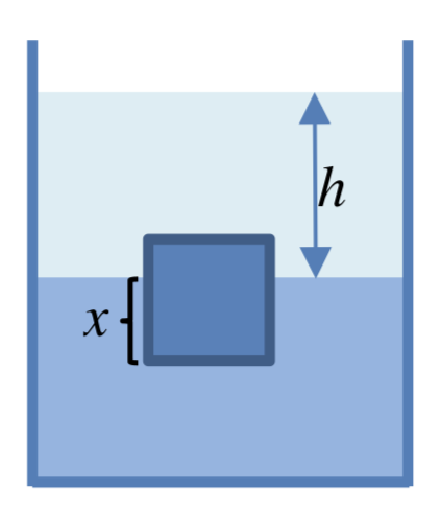
\includegraphics[width=0.7\linewidth]{lahenduskuup}%
\end{center}
\vspace{-10 pt}%
\end{wrapfigure}

\emph{Lahendus 1}\\
Kehale mõjub kolm jõudu - raskusjõud, vedeliku rõhk ülemisele pinnale ja vedeliku rõhk alumisele pinnale: $mg + F_1 - F_2 = 0$\quad (1)
\[ mg = \rho_k l^3g\]
\[ \quad\quad F_1 = \rho_1 g(h - (l-x))l^2, \quad F_2 = \rho_1ghl^2 + \rho_2gxl^2, \]
kus $h$ – väiksema tihedusega vedelikukihi paksus, $x$ – kuubi selle osa pikkus, mis asub suurema tihedusega vedelikus.\\ 
Asendame need jõud seosesse (1). Pärast taandamisi saame seose
\[ (\rho_k - \rho_1)l = (\rho_2 - \rho_1)x \hence x = \SI{7,5}{cm} \]


\emph{Lahendus 2}\\
Vedelikus heljuva keha korral võrdub kehale mõjuv raskusjõud kummagi vedeliku poolt mõjuvate üleslükkejõudude summaga
\[ mg = F_{y2} + F_{y1}, \quad\text{seega} \]
\[ \rho_kl^3g = \rho_2gxl^2 + \rho_1g(l-x)l^2, \hence x=\frac{(\rho_k - \rho_1)l}{(\rho_2 - \rho_1)} = \SI{7,5}{cm}. \]
\fi
}